%% Estructura principal para un reporte de Trabajos intersemanales CIRCAE %%
%% Autor: Edison Abado Ancco ---------------------------------------------%%
\documentclass[a4paper]{IEEEtran} %tamaño del papel y el tipo de transcripción que será IEEE
%\usepackage[total={6.5in,10in},left=1in,top=0.5in,includehead,includefoot]{geometry}
\usepackage[utf8]{inputenc} %el tipo de codificación que incluye símbolos como la tilde
\usepackage[spanish]{babel} % hacemos que nuestro documentación vaya en español
\usepackage{cite} % citas bibliográficas
\usepackage{graphicx} %gráficos, usaremos solo .jpg o .png con estándares que ya veremos
\usepackage{subfigure} %usar subfiguras
\usepackage{url} %agregar direcciones url
\usepackage{amsmath} %expresiones matemáticas
\newtheorem{teor}{Teorema}[section] %definimos la enumeración de Teoremas usando la etiqueta \begin{teor} ... \end{teor} para los ejemplos, podemos darle etiquetas para referenciarlas a lo largo del texto
\newtheorem{ejem}{Ejemplo}[section] %definimos la enumeración de Ejemplos usando la etiqueta \begin{ejem} ... \end{ejem} para los ejemplos, podemos darle etiquetas para referenciarlas a lo largo del texto
\newtheorem{exper}{Experimento}[section] %definimos la enumeración de Ejemplos usando la etiqueta \begin{exper} ... \end{exper} para los Experimentos, podemos darle etiquetas para referenciarlas a lo largo del texto
\usepackage{setspace} %LA usamos para asignar el interlineado
%%%%%%% settings para incluir codigo fuente en cualquier lenguaje
\usepackage{listings} %comenzamos la configuración de nuestras lineas de codigo que se incluirá de ser necesario en el documento
\usepackage[usenames]{color} %seteamos el uso de nombre y color
\definecolor{gray97}{gray}{.97}%definimos nombre y color
\usepackage{textcomp}
\lstset{
	frame=Ltb,
	framerule=1pt,
	framextopmargin=5pt, %margen de arriba
	framexbottommargin=5pt, %margen de abajo
	framexleftmargin= 2pt, %separacion del margen izquierdo
	framesep=5pt,
	rulesep=0.3pt,
	backgroundcolor=\color{gray97},
	rulesepcolor=,
	tabsize=2,
	rulecolor=\color[RGB]{106, 182, 217}, %AZUL
	upquote=true,
	aboveskip={2\baselineskip}, %despues de la linea de texto
	columns=fixed,
	showstringspaces=false,
	extendedchars=true,
	breaklines=true,
	prebreak = \raisebox{0ex}[0ex][0ex]{\ensuremath{\hookleftarrow}},
	showtabs=false,
	showspaces=false,
	showstringspaces=false,
	basicstyle=\scriptsize\ttfamily\color[RGB]{39, 100, 46}, %Numeros de lineas, simbolos, puntos y coma y demas
	identifierstyle=\ttfamily\color[RGB]{56, 140, 189}, %variables
	commentstyle=\color[RGB]{62, 179, 101}, %comentarios
	stringstyle=\color[RGB]{247, 165, 42}, %impresiones
	keywordstyle=\bfseries\color[RGB]{237, 118, 150}, %funciones
	%
	numbers=left,
	numbersep=1pt, %separacion del numero
	numberstyle=\tiny,
	numberfirstline = false,
	breaklines=true,
}
\usepackage{graphicx}
\usepackage[colorinlistoftodos]{todonotes}
\usepackage{enumitem}

\usepackage{feynmp}
\DeclareGraphicsRule{*}{mps}{*}{}

\usepackage{tikz-feynman}
\tikzfeynmanset{compat=1.1.0}
%%%%%%%
\providecommand{\keywords}[1]{\textbf{\textit{Términos Clave---}} #1}

\begin{document}
%	\spacing{0.9} %definimos un interlineado de 0.9 para todo el documento
	
	\title{Filtros Típicos para Rectificadores}
	\author{ING. JUAN PABLO VIZCARDO ZUNIGA, DOCENTE, EDISON ABADO ANCCO, ALUMNO
		}
	
	\markboth{UNIVERSIDAD NACIONAL DE SAN ANTONIO ABAD DEL CUSCO - INGENIERÍA ELECTRÓNICA - LABORATORIO DE CIRCUITOS ELECTRÓNICOS I I - 2021 I -G4-P1-003}{} % Codigo del informe que corresponde a: - numero de grupo con la G antepuesta - numero de proyecto con la P antepuesta | número de informe
	\maketitle
	
	
\begin{abstract}
		La función básica de un rectificador de media u onda completa es llevar una fuente alterna para un uso en DC. La salida rizada debe tener un rizo mínimo y estable sin pícos pronunciados al inicio, y usando componentes pasivos R y L mesurados, los cuales lleven valores comerciales accesibles.\\
		\keywords{\textbf{rectificador, rizo}}
\end{abstract}
	
	
\section{Procedimiento de Laboratorio}

%%%%%%%%%%%%%%%%%%%%%%%%%%%%%%%%%%%%%%%%%%%%%%%%%%%%%%%%%%%%%%%%%%%%%%%%%%
%%%%%%
%%%%%%    PREGUNTA 1
%%%%%%
%%%%%%%%%%%%%%%%%%%%%%%%%%%%%%%%%%%%%%%%%%%%%%%%%%%%%%%%%%%%%%%%%%%%%%%%%%

\subsection{Obtenga las siguientes relaciones teóricas para el rectificador de media onda con filtro de condensador}

\subsubsection{Voltaje de rizado $V_r$}

El voltaje de rizado es la tensión pico pico en la salida filtrada. Ver figura \eqref{rizado1} que es la salida de un filtrado con condensador. Matemáticamente se puede expresar como:

\begin{equation}
	V_r = \frac{V_m}{fR_L C}
\end{equation}

Dado que el circuito rectificador es uno donde el capacitor está en paralelo a la carga $R_L$, entonces el voltaje de rizado también se puede expresar como:

\begin{equation}
	V_r = \frac{I_{dc}}{fC}
\end{equation}

\begin{figure}[h!]
	\centering
	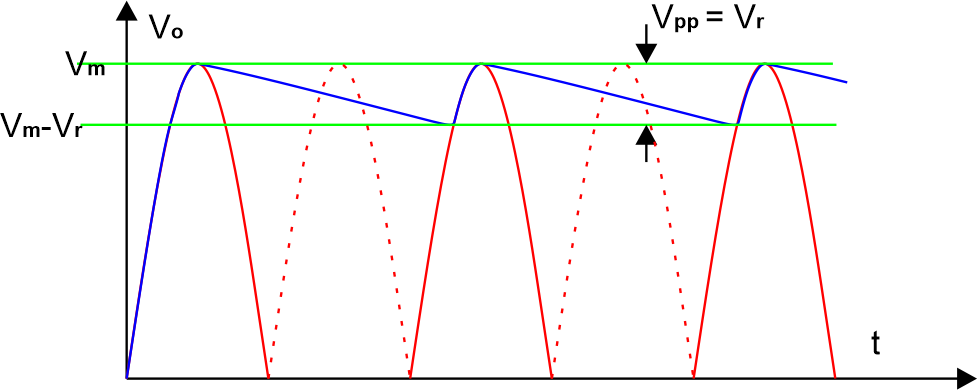
\includegraphics[scale=1]{IMAGENES/rizado1}
	\caption{Voltaje de rizado para media onda.}
	\label{rizado1}
\end{figure}



\subsubsection{Factor de rizado $r$}

Para poder definir matemáticamente el factor de rizado, usamos a la tensión de salida $V_{o,rms}$:

\begin{equation}
	V_{o,rms} = \frac{V_r}{2 \sqrt{3}} = \frac{I_{dc}}{2 \sqrt{3} fC}
\end{equation}

Por lo tanto el factor de rizado queda como:

\begin{equation}
	\label{frizado_media}
	r = \frac{V_{o,rms}}{V_{cd}} = \frac{I_{dc}/2\sqrt{3} fC}{I_{dc} R_L} = \frac{1}{2 \sqrt{3} f C R_L}
\end{equation}

%%%%%%%%%%%%%%%%%%%%%%%%%%%%%%%%%%%%%%%%%%%%%%%%%%%%%%%%%%%%%%%%%%%%%%%%%%
%%%%%%
%%%%%%    PREGUNTA 2
%%%%%%
%%%%%%%%%%%%%%%%%%%%%%%%%%%%%%%%%%%%%%%%%%%%%%%%%%%%%%%%%%%%%%%%%%%%%%%%%%

\subsection{Obtenga las siguientes relaciones teóricas para el rectificador de onda completa con filtro de condensador}

\subsubsection{Voltaje de rizado $V_r$}

El voltaje de rizado es la tensión pico pico en la salida filtrada. Ver figura \eqref{rizado2} que es la salida de un filtrado con condensador. Matemáticamente se puede expresar como:

\begin{equation}
	V_r = \frac{V_m}{2fR_L C}
\end{equation}

Dado que el circuito rectificador es uno donde el capacitor está en paralelo a la carga $R_L$, entonces el voltaje de rizado también se puede expresar como:

\begin{equation}
	V_r = \frac{I_{dc}}{2fC}
\end{equation}

\begin{figure}[h!]
	\centering
	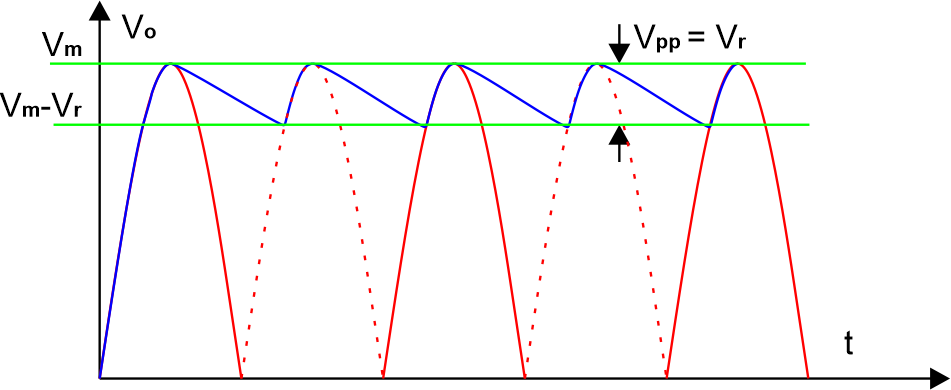
\includegraphics[scale=1]{IMAGENES/rizado2}
	\caption{Voltaje de rizado para onda completa.}
	\label{rizado2}
\end{figure}



\subsubsection{Factor de rizado $r$}

Para poder definir matemáticamente el factor de rizado, usamos a la tensión de salida $V_{o,rms}$:

\begin{equation}
	V_{o,rms} = \frac{V_r}{2 \sqrt{3}} = \frac{I_{dc}}{4 \sqrt{3} fC}
\end{equation}

Por lo tanto el factor de rizado queda como:

\begin{equation}
	\label{frizado_completa}
	r = \frac{V_{o,rms}}{V_{cd}} = \frac{I_{dc}/4\sqrt{3} fC}{I_{dc} R_L} = \frac{1}{4 \sqrt{3} f C R_L}
\end{equation}

%%%%%%%%%%%%%%%%%%%%%%%%%%%%%%%%%%%%%%%%%%%%%%%%%%%%%%%%%%%%%%%%%%%%%%%%%%
%%%%%%
%%%%%%    PREGUNTA 3
%%%%%%
%%%%%%%%%%%%%%%%%%%%%%%%%%%%%%%%%%%%%%%%%%%%%%%%%%%%%%%%%%%%%%%%%%%%%%%%%%

\subsection{¿Por qué es recomendable contar con una resistencia de purga?}

Por que puede suceder que la carga se desconecte en elgún momento, y esta situación dejaría al capacitor totalmente cargado por tiempo indefinido. Para ello es necesario integrar una resistencia alta (denominada resistencia de purga de alrededor de 1M$\Omega$ a 10M$\Omega$) para que cuando la carga esté desconectada, el capacitor no represente riesgo alguno.

%%%%%%%%%%%%%%%%%%%%%%%%%%%%%%%%%%%%%%%%%%%%%%%%%%%%%%%%%%%%%%%%%%%%%%%%%%
%%%%%%
%%%%%%    PREGUNTA 4
%%%%%%
%%%%%%%%%%%%%%%%%%%%%%%%%%%%%%%%%%%%%%%%%%%%%%%%%%%%%%%%%%%%%%%%%%%%%%%%%%

\subsection{En un rectificador LC, ¿Cuál es el valor de la inductancia critica LC?}

Dado que la tensión media de la bobina en regimen permanente (ver figura \eqref{rectificador}) es cero, el voltaje medio de salida es:

\begin{figure}[h!]
	\centering
	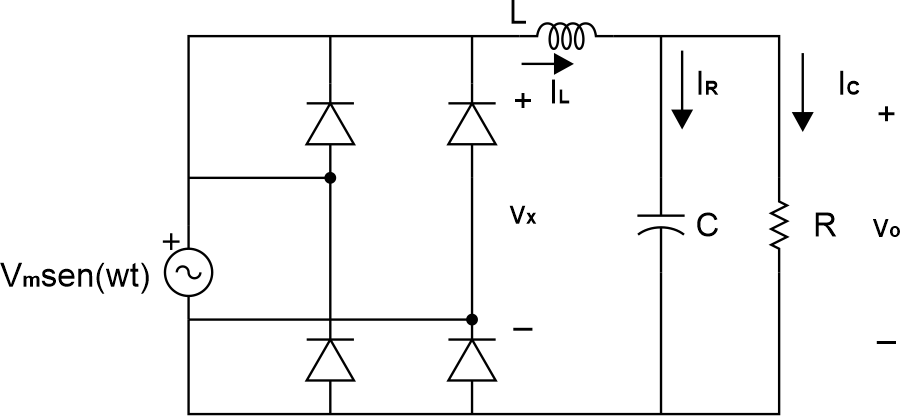
\includegraphics[scale=1]{IMAGENES/rectificador}
	\caption{Voltaje de rizado para onda completa.}
	\label{rectificador}
\end{figure}

\begin{equation}
	V_o = \frac{2 V_m}{\pi}
\end{equation}

La corriente media de la bobina es igual a la de la resistencia, porque la corriente media del capacitor es cero.

\begin{equation}
	I_L = I_R = \frac{V_o}{R} = \frac{2V_m}{\pi R}
\end{equation}

Podemos estimar la vartiacion de corriente en la bobina del primer término en alterna de la serie de fourier.


\begin{equation}
	v_o(\omega t) = V_o + \sum_{n = 2,4,6,...}^{\infty} V_n cos(n\omega t + \pi)
\end{equation}

donde $V_o = \frac{2V_n}{\pi}$ y $V_n = \frac{2V_m}{\pi} \left(\frac{1}{n-1} - \frac{1}{n+1}\right)$; para $n = 2$, y suponiendo que el capacitor es u cortocircuito en alterna, tendrémos un armónico $v_2$ en la bobina. La amplitud de la corriente de la bobina para $n=2$:

\begin{equation}
	I_2 = \frac{V_2}{Z_2} \simeq \frac{V_2}{2 \omega L} = \frac{4V_m / 3 \pi}{2 \omega L} = \frac{2 V_m}{3 \pi \omega L}
\end{equation}

Para que la corriente sea siempre positiva, la amplitud del término en alterna deberá ser menor que la del término en continua (valor medio).

\begin{equation}
	I_2 < I_L
\end{equation}

Reemplazando $\frac{2V_m}{3 \pi \omega L} < \frac{2V_m}{\pi R}$, por lo que:

\begin{equation}
	\label{lcCritica}
	L < \frac{R}{3 \omega}
\end{equation}

Por lo que podemos decir que nuestra inductancia crítica $L_c$ estará dada por la ecuación anterior. Valores por debajo de esta variable serán adecuadas.

%%%%%%%%%%%%%%%%%%%%%%%%%%%%%%%%%%%%%%%%%%%%%%%%%%%%%%%%%%%%%%%%%%%%%%%%%%
%%%%%%
%%%%%%    PREGUNTA 5
%%%%%%
%%%%%%%%%%%%%%%%%%%%%%%%%%%%%%%%%%%%%%%%%%%%%%%%%%%%%%%%%%%%%%%%%%%%%%%%%%

\subsection{Graficar formas de onda para el circuito rectificador de media onda.}

Dado el circuito de la imagen \eqref{a50}, graficar las formas de onda para $C = 10\mu F$. Estas curvas se muestran en la figura \eqref{a51}

\begin{figure}[h!]
	\centering
	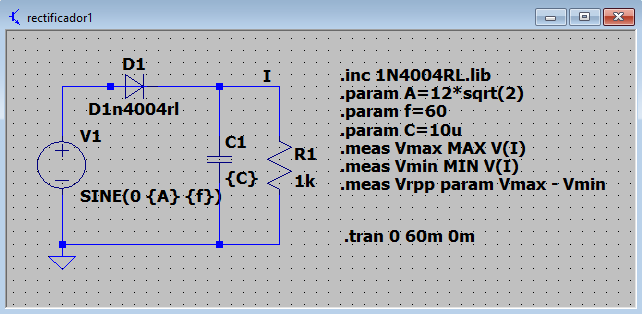
\includegraphics[scale=0.5]{IMAGENES/a50}
	\caption{Circuito Rectificador de Media Onda.}
	\label{a50}
\end{figure}

\begin{figure}[h!]
	\centering
	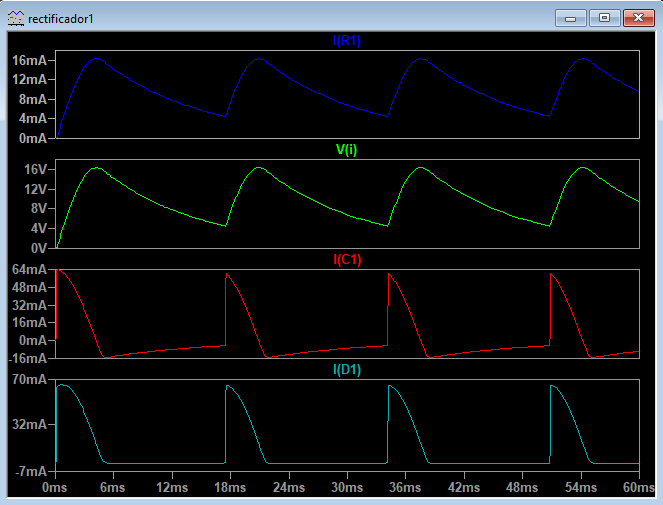
\includegraphics[scale=0.5]{IMAGENES/a51}
	\caption{Forma de onda de la tensión de carga, corriente de carga, corriente que pasa por C1 y corriente que pasa por D1.}
	\label{a51}
\end{figure}

El voltaje de rizado usando las directivas .MEAS MAX MIN es de $V=11.8136V$ (ver figura \eqref{a52}), el cual es un valor muy alto. Para un mejor desempeño tendremos que variar la capacitancia.

\begin{figure}[h!]
	\centering
	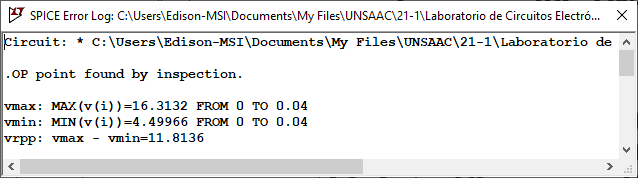
\includegraphics[scale=0.5]{IMAGENES/a52}
	\caption{Ventana de Error log Para ver el voltaje de rizado usando las directivas .meas.}
	\label{a52}
\end{figure}



\begin{figure}[h!]
	\centering
	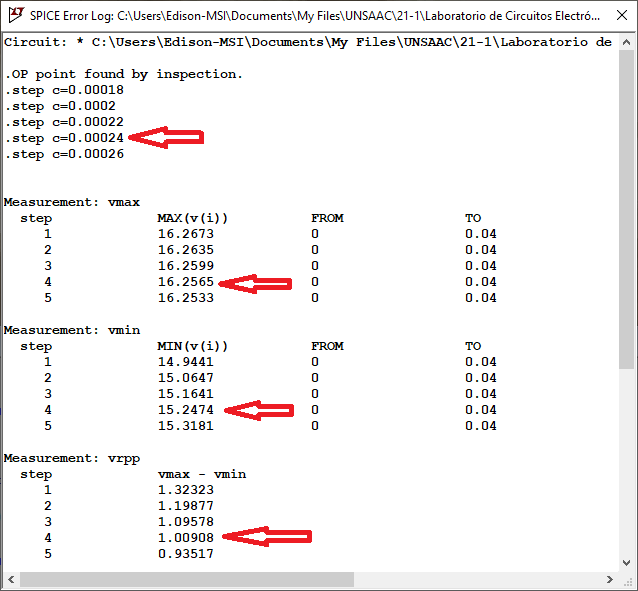
\includegraphics[scale=0.5]{IMAGENES/a53}
	\caption{Ventana de Error log Para ver el voltaje de rizado usando las directivas .meas y .step para hallar un $C$ adecuado que pueda generar un $V_r \simeq 1.0V$}
	\label{a53}
\end{figure}

Variando el Valor de C para obtener un voltaje de rizado de $1V_{pp}$, y usando las directivas .step y .meas tendremos el resultado que muestra la imagen \eqref{a53}. En el podemos ver que $V_r = 1.009V$ para $C = 240uF$. Este resultado es un resultado aproximado, y es aceptable, hay un margen de error pequeño.

Ahora graficamos y generamos las curvas correspondientes a $C=240uF$, como se muestra en la figura \eqref{a54}.

\begin{figure}[h!]
	\centering
	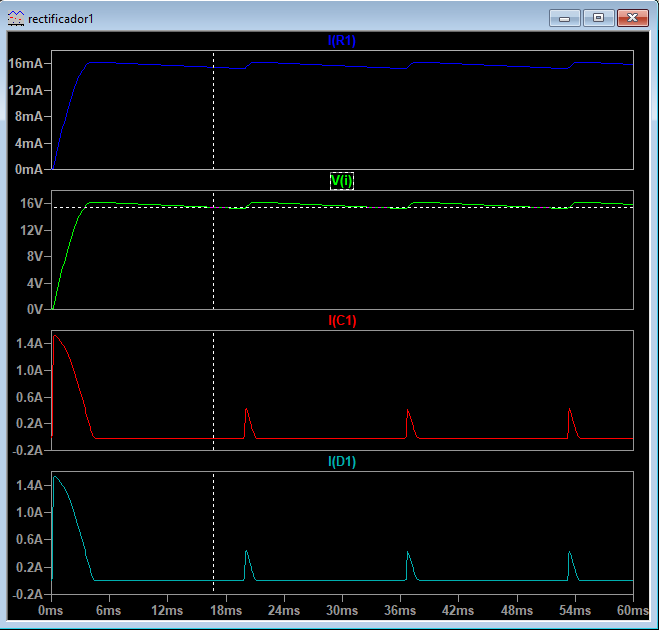
\includegraphics[scale=0.5]{IMAGENES/a54}
	\caption{Forma de onda de la tensión de carga, corriente de carga, corriente que pasa por C1 y corriente que pasa por D1.}
	\label{a54}
\end{figure}

%%%%%%%%%%%%%%%%%%%%%%%%%%%%%%%%%%%%%%%%%%%%%%%%%%%%%%%%%%%%%%%%%%%%%%%%%%
%%%%%%
%%%%%%    PREGUNTA 6
%%%%%%
%%%%%%%%%%%%%%%%%%%%%%%%%%%%%%%%%%%%%%%%%%%%%%%%%%%%%%%%%%%%%%%%%%%%%%%%%%

\subsection{Graficar formas de onda para el circuito rectificador de onda completa.}

Se tiene el circuito de la figura \eqref{a60}. Para el cual se debe elegir un $C$ adecuado que genere un $Vr = 0.2V_{pp}$.

\begin{figure}[h!]
	\centering
	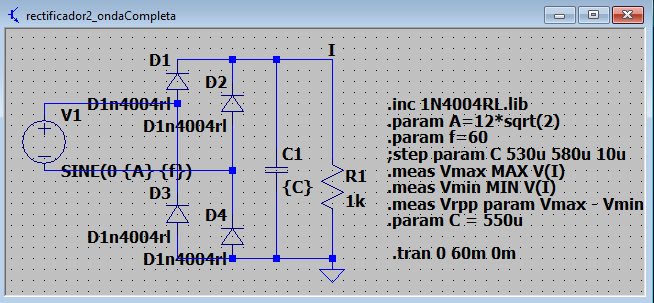
\includegraphics[scale=0.5]{IMAGENES/a60}
	\caption{Circuito rectificador de Onda completa.}
	\label{a60}
\end{figure}

Para ello usamos las directivas .step y .meas que generarán los datos de la figura \eqref{a61}, según el cual, podemos aproximar un $C=550uF$ para obtener $V_r = 0.201742V \simeq 0.2V_{pp}$

\begin{figure}[h!]
	\centering
	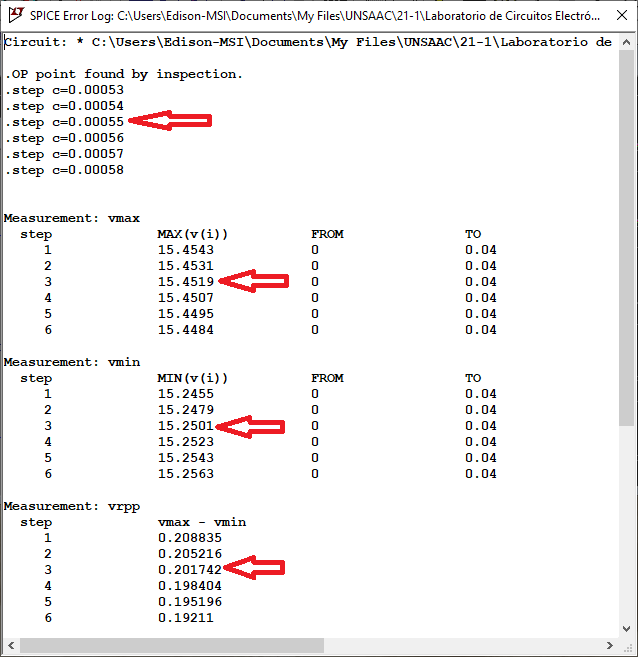
\includegraphics[scale=0.5]{IMAGENES/a61}
	\caption{Ventana de Error log Para ver el voltaje de rizado usando las directivas .meas y .step.}
	\label{a61}
\end{figure}

Seguidamente graficamos las curvas correspondientes para $C=550uF$, ver figura \eqref{a62}.

\begin{figure}[!h]
	\centering
	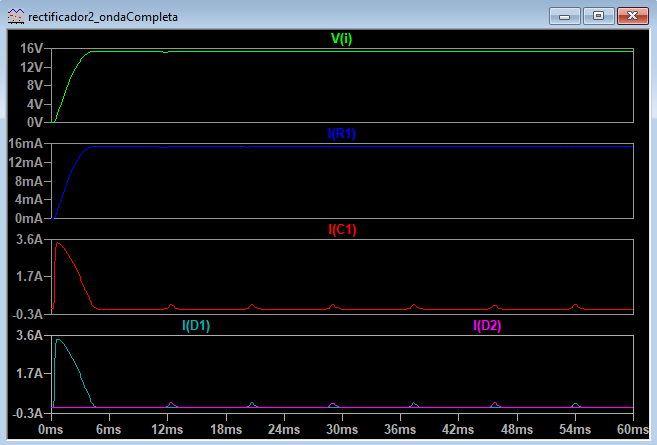
\includegraphics[scale=0.5]{IMAGENES/a62}
	\caption{Forma de onda de la tensión de carga, corriente de carga, corriente que pasa por C1, corrientes que pasan por D1 y D2 con $C = 550uF$ y $R_L = 1k\Omega$.}
	\label{a62}
\end{figure}

Ahora, si variamos el valor de la Carga a $R_L = 100 \Omega$, tengramos las curvas que se muestran en la figura \eqref{a63}.

\begin{figure}[!h]
	\centering
	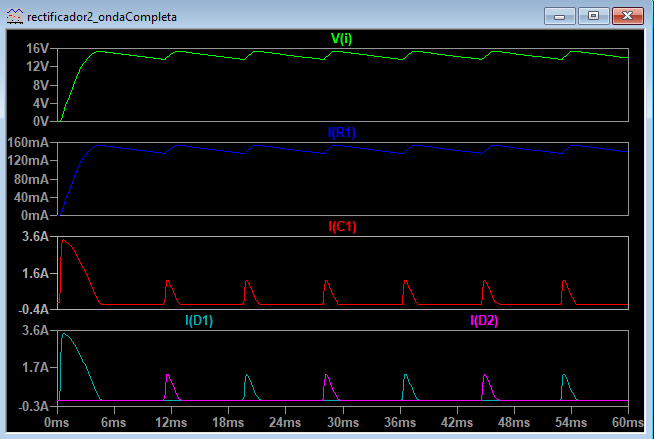
\includegraphics[scale=0.5]{IMAGENES/a63}
	\caption{Forma de onda de la tensión de carga, corriente de carga, corriente que pasa por C1, corrientes que pasan por D1 y D2 Para $C = 550uF$ y una carga variada a $R_L = 100 \Omega$.}
	\label{a63}
\end{figure}

Hallamos el $V_r$ usando las directivas .meas MAX MIN (ver figura \eqref{a64}), el cual muestra que  $V_r = 1.75222V$.

\begin{figure}[!h]
	\centering
	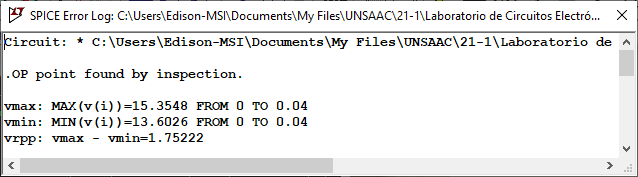
\includegraphics[scale=0.5]{IMAGENES/a64}
	\caption{$V_r$ para $C = 550uF$, $R_L = 100\Omega$.}
	\label{a64}
\end{figure}

%%%%%%%%%%%%%%%%%%%%%%%%%%%%%%%%%%%%%%%%%%%%%%%%%%%%%%%%%%%%%%%%%%%%%%%%%%
%%%%%%
%%%%%%    PREGUNTA 7
%%%%%%
%%%%%%%%%%%%%%%%%%%%%%%%%%%%%%%%%%%%%%%%%%%%%%%%%%%%%%%%%%%%%%%%%%%%%%%%%%

\subsection{¿El valor del voltaje de rizado depende de resistencia de carga? (sustentar)}

De manera experimental podemos ver que $V_r$ si depende de la carga, cuando no variamos los parámetros de $C$, y aumentamos el valor por encima de $1k\Omega$ por ejemplo, $V_r$ disminuye, y si disminuimos el valor de $R_L$, $V_r$ aumenta.
Matemáticamente podemos ver, de acuerdo a las ecuaciones \eqref{frizado_completa} y \eqref{frizado_media}, que señalan los factores de rizado de media y onda completa, muestran una relación inversa entre el factor de rizado con la carga $R_L$, por lo que es lógico el comportamiento de $V_r$ en el análisis experimental.

%%%%%%%%%%%%%%%%%%%%%%%%%%%%%%%%%%%%%%%%%%%%%%%%%%%%%%%%%%%%%%%%%%%%%%%%%%
%%%%%%
%%%%%%    PREGUNTA 8
%%%%%%
%%%%%%%%%%%%%%%%%%%%%%%%%%%%%%%%%%%%%%%%%%%%%%%%%%%%%%%%%%%%%%%%%%%%%%%%%%

\subsection{Para el circuito de la figura \eqref{a60} elegir $L_c$ (inductancia crítica) y $C$ para obtener el mismo rizado de 0.2Vpp}

De la ecuación \eqref{lcCritica} podemos calcular que $L_c = \frac{R_L}{3\omega}$. Tenemos que $R_L = 1k\Omega$, por lo que $L_c = 1\Omega / 3(2*2*\pi*60) \simeq 442mH$. Para hallar la $C$ correcta para $V_r = 0.2V_{pp}$ usamos las directivas .meas y .step (Ver figura \eqref{a71}), en donde encontramos que $C= 220uF$ para $V_r = 0.205976V_{pp}$.

\begin{figure}[!h]
	\centering
	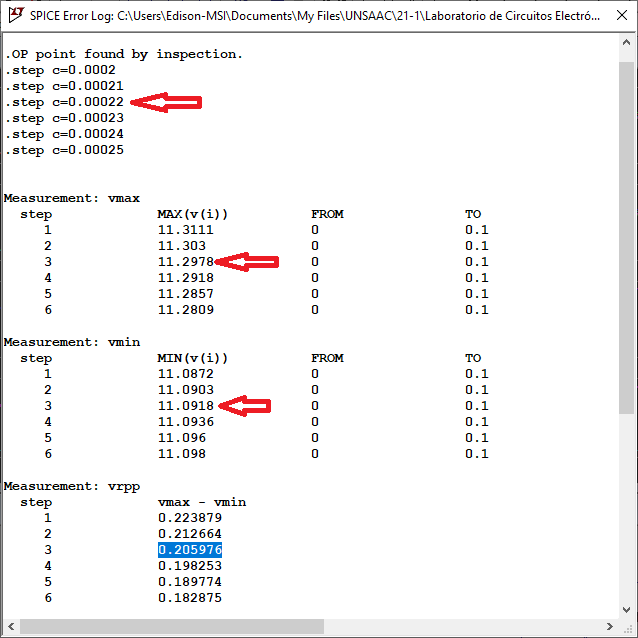
\includegraphics[scale=0.5]{IMAGENES/a71}
	\caption{$V_r$ para $L_c = 442mH$, $C = 220uF$, $R_L = 1k\Omega$.}
	\label{a71}
\end{figure}

\begin{figure}[!h]
	\centering
	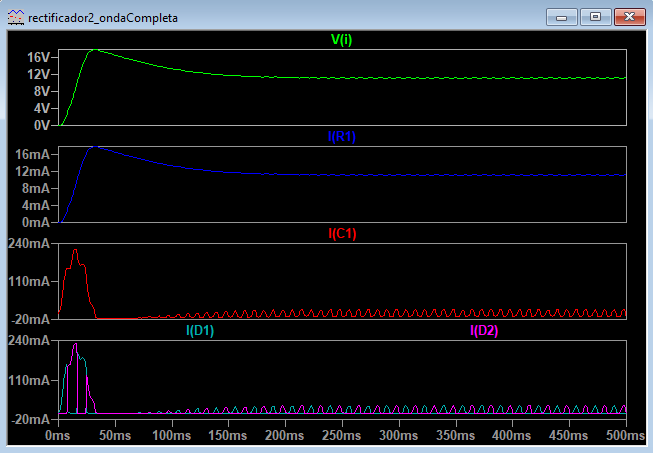
\includegraphics[scale=0.5]{IMAGENES/a72}
	\caption{Forma de onda de la tensión de carga, corriente de carga, corriente que pasa por C1, corrientes que pasan por D1 y D2 para $L_c = 442mH$, $C = 220uF$, $R_L = 1k\Omega$.}
	\label{a72}
\end{figure}

Las corrientes pico en los diodos disminuye notablemente, esto debido al comportamiento fundamental del inductor, que almacena energía en forma de campo magnético generado por la corriente eléctrica que pasa por ella. 
El comportamiento más notable en el circuito de experimentaci;on es que sin el inductor, la corriente pico llega a más de3 Amperios, en cambio, con el inductor de valor $L_c$ tan solo tiene una corriente pico de menos de $240mA$. En contraparte, la corriente y tensión rectificada (en $R_L$), esto se podría arreglar disminuyendo el valor de $L$, hasta tener un balance entre corrientes pico y niveles de tensión y corriente aceptables en $R_L$.

%%%%%%%%%%%%%%%%%%%%%%%%%%%%%%%%%%%%%%%%%%%%%%%%%%%%%%%%%%%%%%%%%%%%%%%%%%
%%%%%%
%%%%%%    PREGUNTA 9
%%%%%%
%%%%%%%%%%%%%%%%%%%%%%%%%%%%%%%%%%%%%%%%%%%%%%%%%%%%%%%%%%%%%%%%%%%%%%%%%%

\subsection{Para el circuito de la figura \eqref{a60} diseñar un circuito CLC para obtener un rizado de 0.1Vpp}

Para este diseño vemos el circuito de la figura \eqref{a81}, en el que consideramos $L_c = 442mH$, y los capacitores del mismo valor.

\begin{figure}[!h]
	\centering
	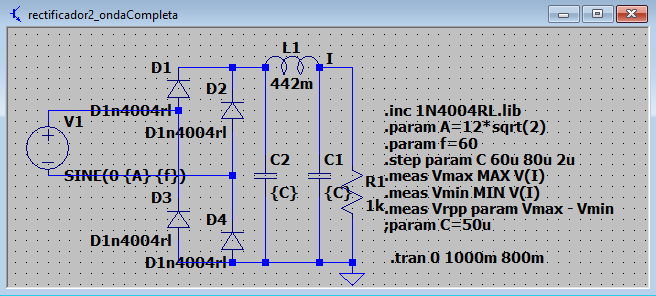
\includegraphics[scale=0.5]{IMAGENES/a81}
	\caption{Circuito CLC Para obtener $V_r = 1V_{pp}$.}
	\label{a81}
\end{figure}

De la figura \eqref{a82} podemos ver que para $C= 70uF$ obtenemos $V_r = 0.102413 V{pp}$, el cual es un valor aceptable.

\begin{figure}[!h]
	\centering
	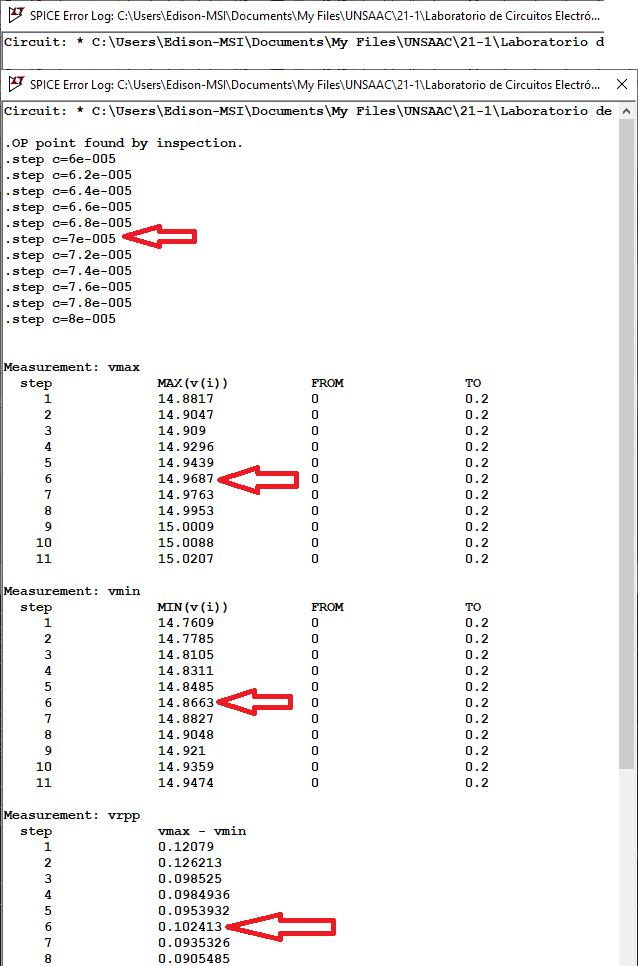
\includegraphics[scale=0.5]{IMAGENES/a82}
	\caption{directivas .step y .meas para hallar un $C$ adecuado para $V_r = 1V_{pp}$.}
	\label{a82}
\end{figure}

Graficamos las curvas correspondientes, en los que podemos ver que $C_2$ tiene picos marcados, pero no de gran magnitud, $C_1$ ya no tiene esos picos marcados, es mucho más estable. El comportamiento en los diodos tienen picos de menos de $500mA$, el cual es un valor que los dispositivos (como el de la serie 1N404) pueden soportar. Lo que se observa claramente es un comportamiento oscilatorio hasta el los $100ms$, tiempo desde el cual las curvas muestran un comportamiento estable. 

\begin{figure}[!h]
	\centering
	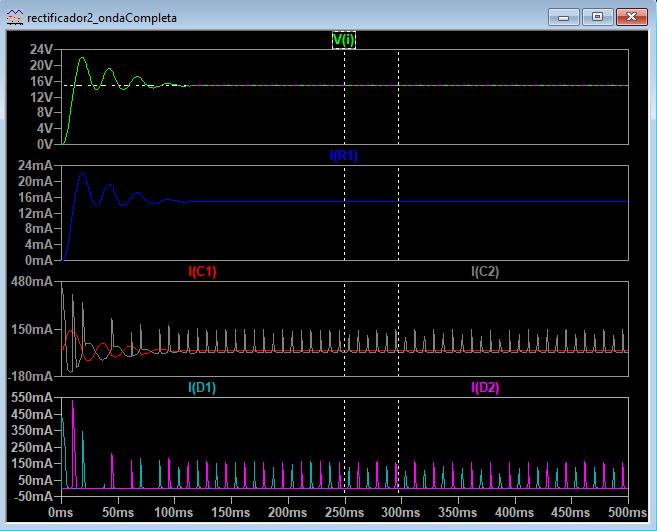
\includegraphics[scale=0.5]{IMAGENES/a83}
	\caption{Forma de onda de la tensión de carga, corriente de carga, corriente que pasa por C1, C2, corrientes que pasan por D1 y D2 para $L_c = 442mH$, $C_{1,2} = 70uF$, $R_L = 1k\Omega$.}
	\label{a83}
\end{figure}



\end{document}

